\section{Brake Pressure Acquisition Channel}\label{sec:brake-pressure-acquisition-channel}

\subsection{Load Cell Signal}\label{ssec:load-cell-signal}

	A very influential parameter in a braking system is the pressure that the brake exerts on the rotor. Pressure is a magnitude measured in Pascal and can be expressed by the force ratio by the area. There are some sensors based on the piezoelectric effect, but the most accurate way to measure force is by using load cells.
	\par
	Load cells have very low output levels, of the level of 2mV/V, and therefore an amplification is fundamental. It is not necessary to know the nature of the strain gauges when a load cell is being calibrated since generally the manufacturers provide a calibration curve based on the signals $V_{O}$ and $V_{EX}$ of the Figure \ref{fig:wheatstone}, it is worth noting that these signals can not have the same reference, otherwise it will not be possible to excite the wheatstone bridge correctly.
	\par
	The most common way to amplify the signal of a load cell is using a instrumentation amplifier. Although it is a widely used configuration, assembling this amplifier using three different operational amplifiers and seven resistors as in Figure \ref{fig:instrumentation-amplifier} may make it inaccurate due to manufacturing imperfections of the components. Another factor that greatly influences the output signal of a load cell is the excitation voltage of its wheatstone bridge, if it varies too much the output will vary greatly as well, which will hamper its calibration.

\subsection{Load Cell Signal Conditioning}\label{ssec:load-cell-signal-conditioning}
		
	In order to solve these two problems there is a solution widely used in the market which is the \textit{AD8223} from Analog Devices \cite{ad8223-datasheet}, this IC is an integrated single supply instrumentation amplifier that delivers rail-to-rail output swing. Other good feature of this amplifier is that as it has a great CMRR (\textit{Common-Mode Rejection Ratio} check Section \ref{itm:opamp-cmrr}) of 80dB, making it very much suitable for condionting differential pair signals (such as the one from the Load Cell as Subsection \ref{ssec:load-cell} mentions), more information of CMRR in Subsection \ref{sssec:important-features-to-consider-in-a-amplifier}. The only external component needed is a resistor $R_{G}$, as shown in Figure \ref{fig:ad8223-schematic}. This resistor will determine the gain (G) for the amplification according to the Equation \ref{eqn:ad8223-g}.
	

		\begin{figure}[htbp]
			\centering
				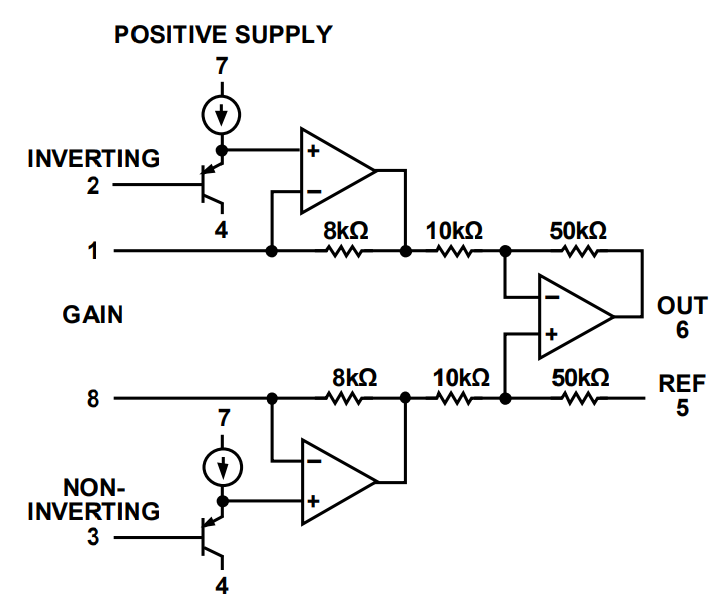
\includegraphics[scale=0.65]{figuras/fig-ad8223-functional-block.png}
			\caption{AD8223 Schematic \cite{ad8223-datasheet}}
			\label{fig:ad8223-schematic}
		\end{figure}

		\begin{equation}\label{eqn:ad8223-g}
			R_{G}=\frac{80k\Omega}{G - 5}
		\end{equation}

		Taking into account the sensitivity of 2mV/V, this means that if the cell is excited with 10V, its output will vary from 0 to 20mV. The precision of the excitation voltage will naturally affect the performance of the sensor, Section \ref{sssec:10v-reference} will explain how a precise 10V voltage reference will be achieved.
		\par
		Since the analog input of the chosen microcontroller \textit{(Atmega328)} is 0 to 5V, we may to amplify the cell output signal by a factor of 250 in order to use the most number of bits from de MCU's ADC. Using Equation \ref{eqn:ad8223-g}, to obtain a gain of amplification ratio of the ideal $R_{G}$ would be 326$\Omega$, a resistor of this value and minimal tolerance (1$\%$) is not commercially available, the closest one is 332$\Omega$. This resistor will generate a gain of 246 and cause the IC output to range from about 0V to 4.92V, using 98.4\% of the resolution of the microcontroller input. 
		\par

		Figure \ref{fig:cic-cell} shows the schematic of the load cell conditioning circuit with the AD8223.

		\begin{figure}[htbp]
			\centering
				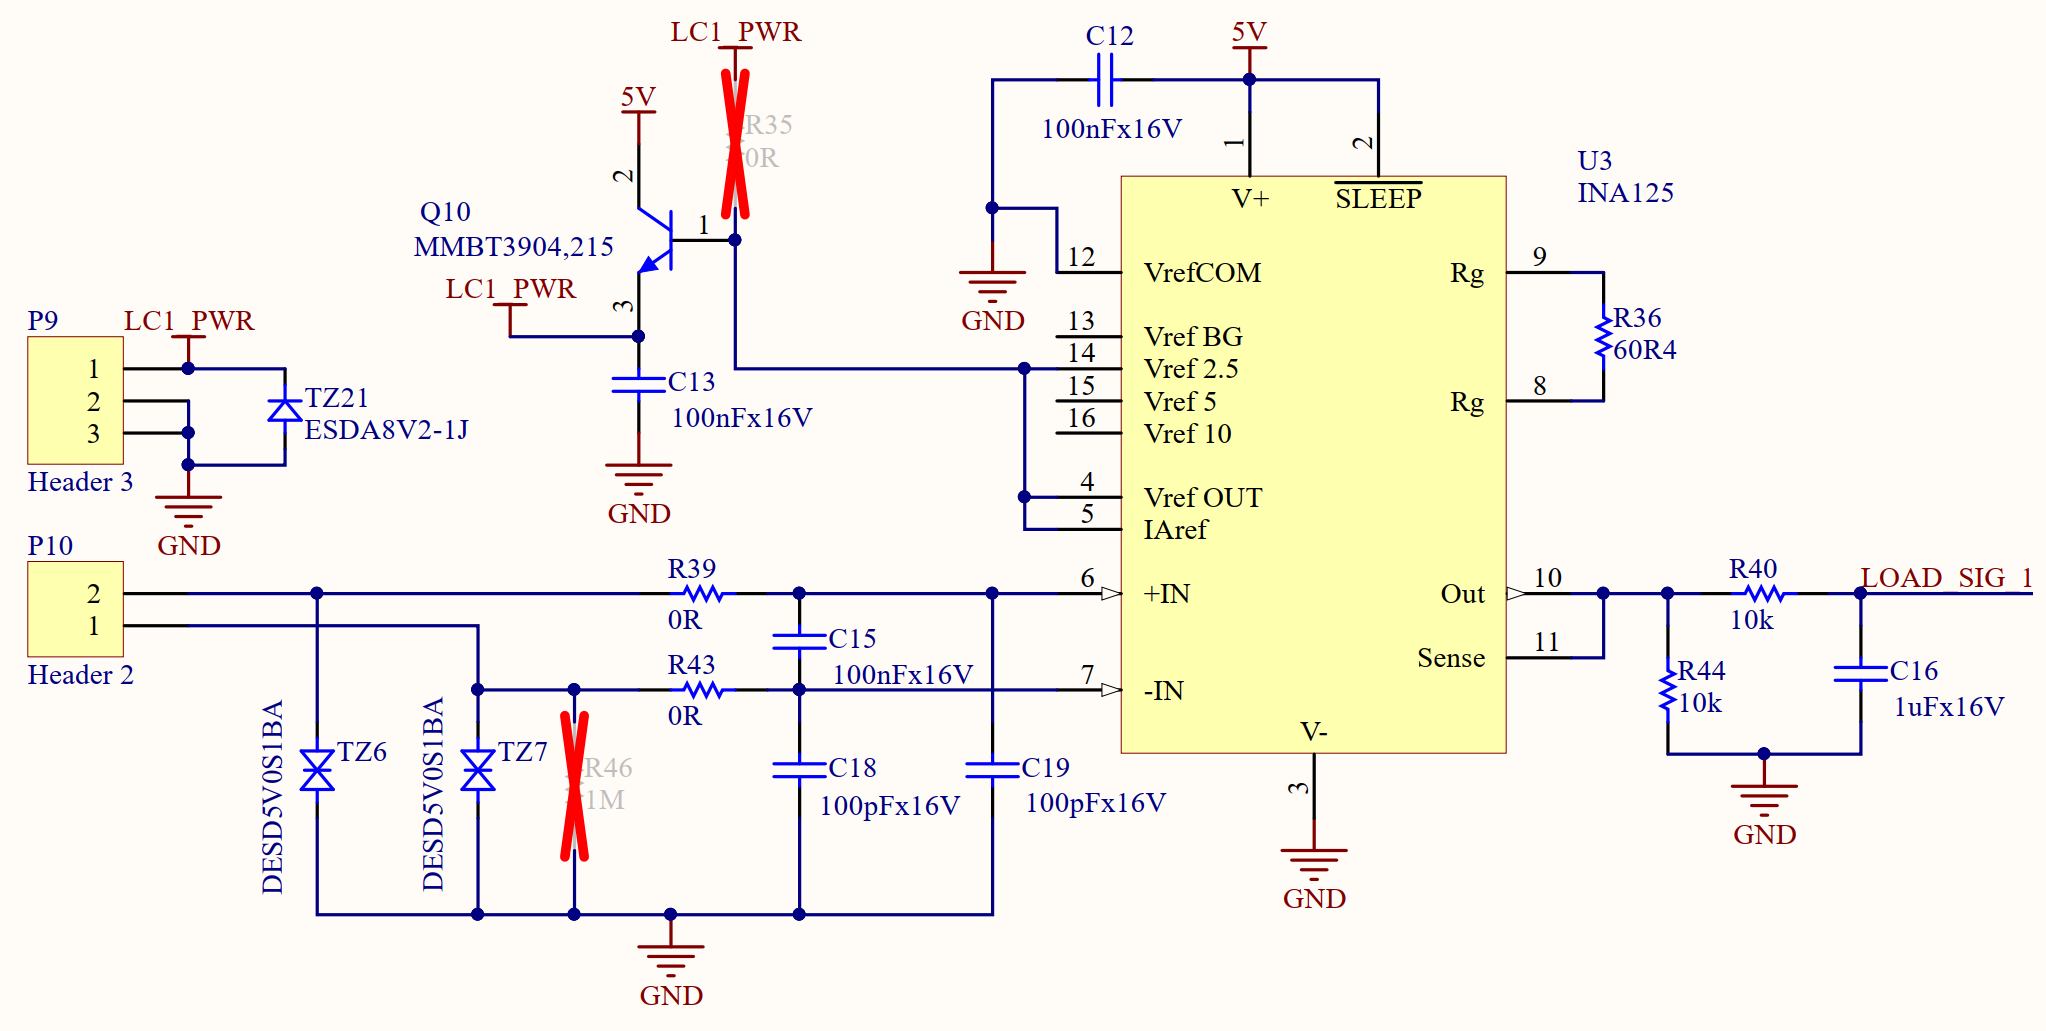
\includegraphics[scale=0.35]{figuras/fig-cic-cell.png}
			\caption{Conditioning Circuit for the Load Cell \cite{conditioning-circuit-for-the-load-cell}}
			\label{fig:cic-cell}
		\end{figure}

		It is basically the amplifier with the gain resistor plus five different types of components:
		\begin{itemize}
			\item \textbf{TVS Diode:} AD8223 datasheet says that the differential input voltage must not be greater than the supply voltage \cite{ad8223-datasheet}, hence, as the supply is 5V, a 5V TVS was added.
			\item \textbf{Decoupling Capacitor:} A decoupling capacitor is recommended by the component's datasheet \cite{ad8223-datasheet}.
			\item \textbf{Resistor R21:} Used to guarantee that if the sensor is disconnected the inverted input will be shunted to GND as according to Figure \ref{fig:ad8223-schematic} the PNP transistors in the non-inverted input will saturate the output to the supply voltage \textit{(this feature is used for detecting when the sensor is disconnected, further explained in Subsection: \ref{ssec:load-cell-sensor-detection}).}
			\item \textbf{R17 and R15:} This jumpers are used just if the need to test circuit blocks separately.
		\end{itemize}

\subsection{Load Cell Sensor Detection}\label{ssec:load-cell-sensor-detection}
	As was explained in Subsection \ref{ssec:load-cell-signal-conditioning}, with R21 the circuit will saturate the output to the supply voltage when the load cell sensor is disconnected. The circuit to detect this voltage saturation is exact the same from the one used previously on the thermocouple circuit, the circuit schematic and functional explanation can be found in Subsection \ref{ssec:thermocouple-sensor-detection}.

	\subsection{Complete Circuit}\label{ssec:load-cell-complete-circuit}
		The thermocouple complete circuit is displayed on Figure \ref{fig:load-cell-complete-circuit}.

		\begin{figure}[htbp]
			\centering
				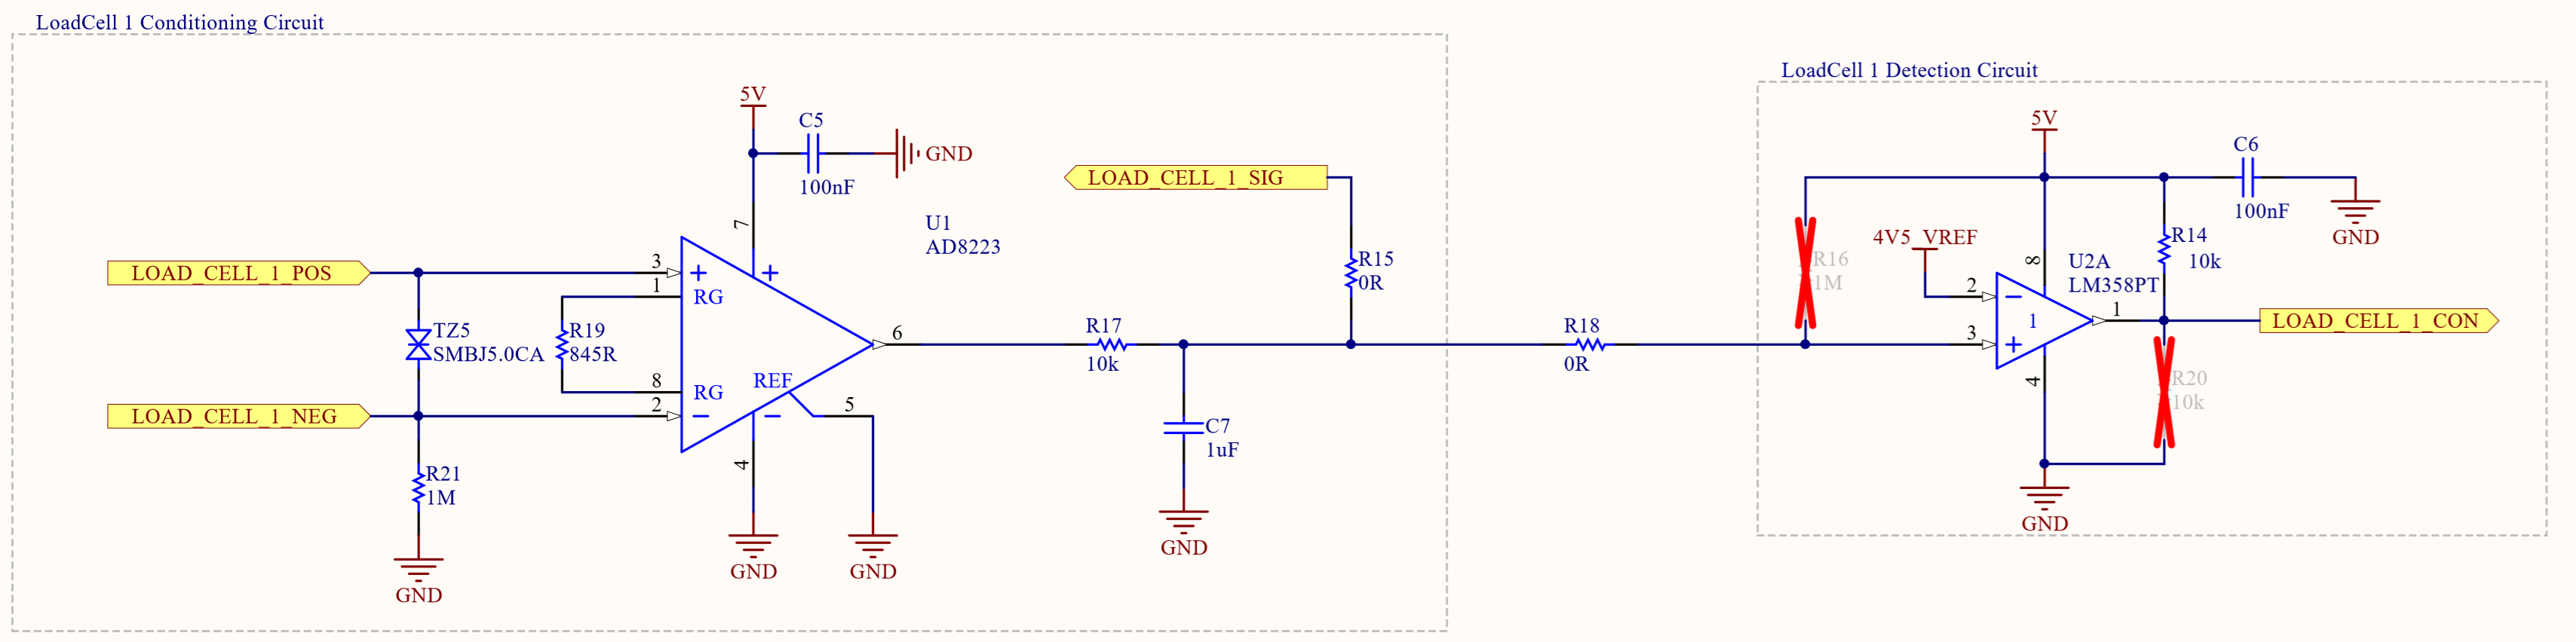
\includegraphics[scale=0.7]{figuras/fig-load-cell-complete-circuit}
			\caption{Load Cell Complete Circuit \cite{load-cell-complete-circuit}}
			\label{fig:load-cell-complete-circuit}
		\end{figure}		

		The pair composed of R17 and C7 is a LFP with a central frequency of 16Hz, used to filter any further noise including the 50/60Hz noise from AC power lines that the thermocouple wires may catch. R15 and R18 were included in case a individual circuit block test is required, both are 0R resistors (jumpers). R20 is just a pull-down to guarantee that the MCU input port will not fluctuate.	